\chapter{Liquid Dynamics}

A non-circularly symmetric molecule on a plane has three degrees of freedom, translations in the $x$ and $y$ directions and a rotation in the $xy$ plane. Understanding the dynamics of a system requires an understanding of the translations and rotations that take place within that system while providing a basis for further study, giving information about the timescales on which events are likely to occur.

\section{Choice of Molecules}

With little prior research into the properties of molecular systems we chose the simplest types of molecules possible, a two particle dimer~\figref{dimer} and a three particle trimer~\figref{trimer}. The simplicity of these molecules allow us to survey a range of different molecular parameters to find molecules of interest for further study in this thesis. The survey included both the Dimer and Trimer molecule types over a radius range $r = [0.5,1]$, a distance range of $d = [1,1+r]$ and an angle range of $\theta = [90^\circ,180^\circ]$. These ranges were chosen so the resulting molecules are sufficiently distinct from a disc, a problem that has been studied for a long time~\cite{verlet:67}.

\begin{figure}
    \centering
    \begin{subfigure}[t]{0.48\textwidth}
        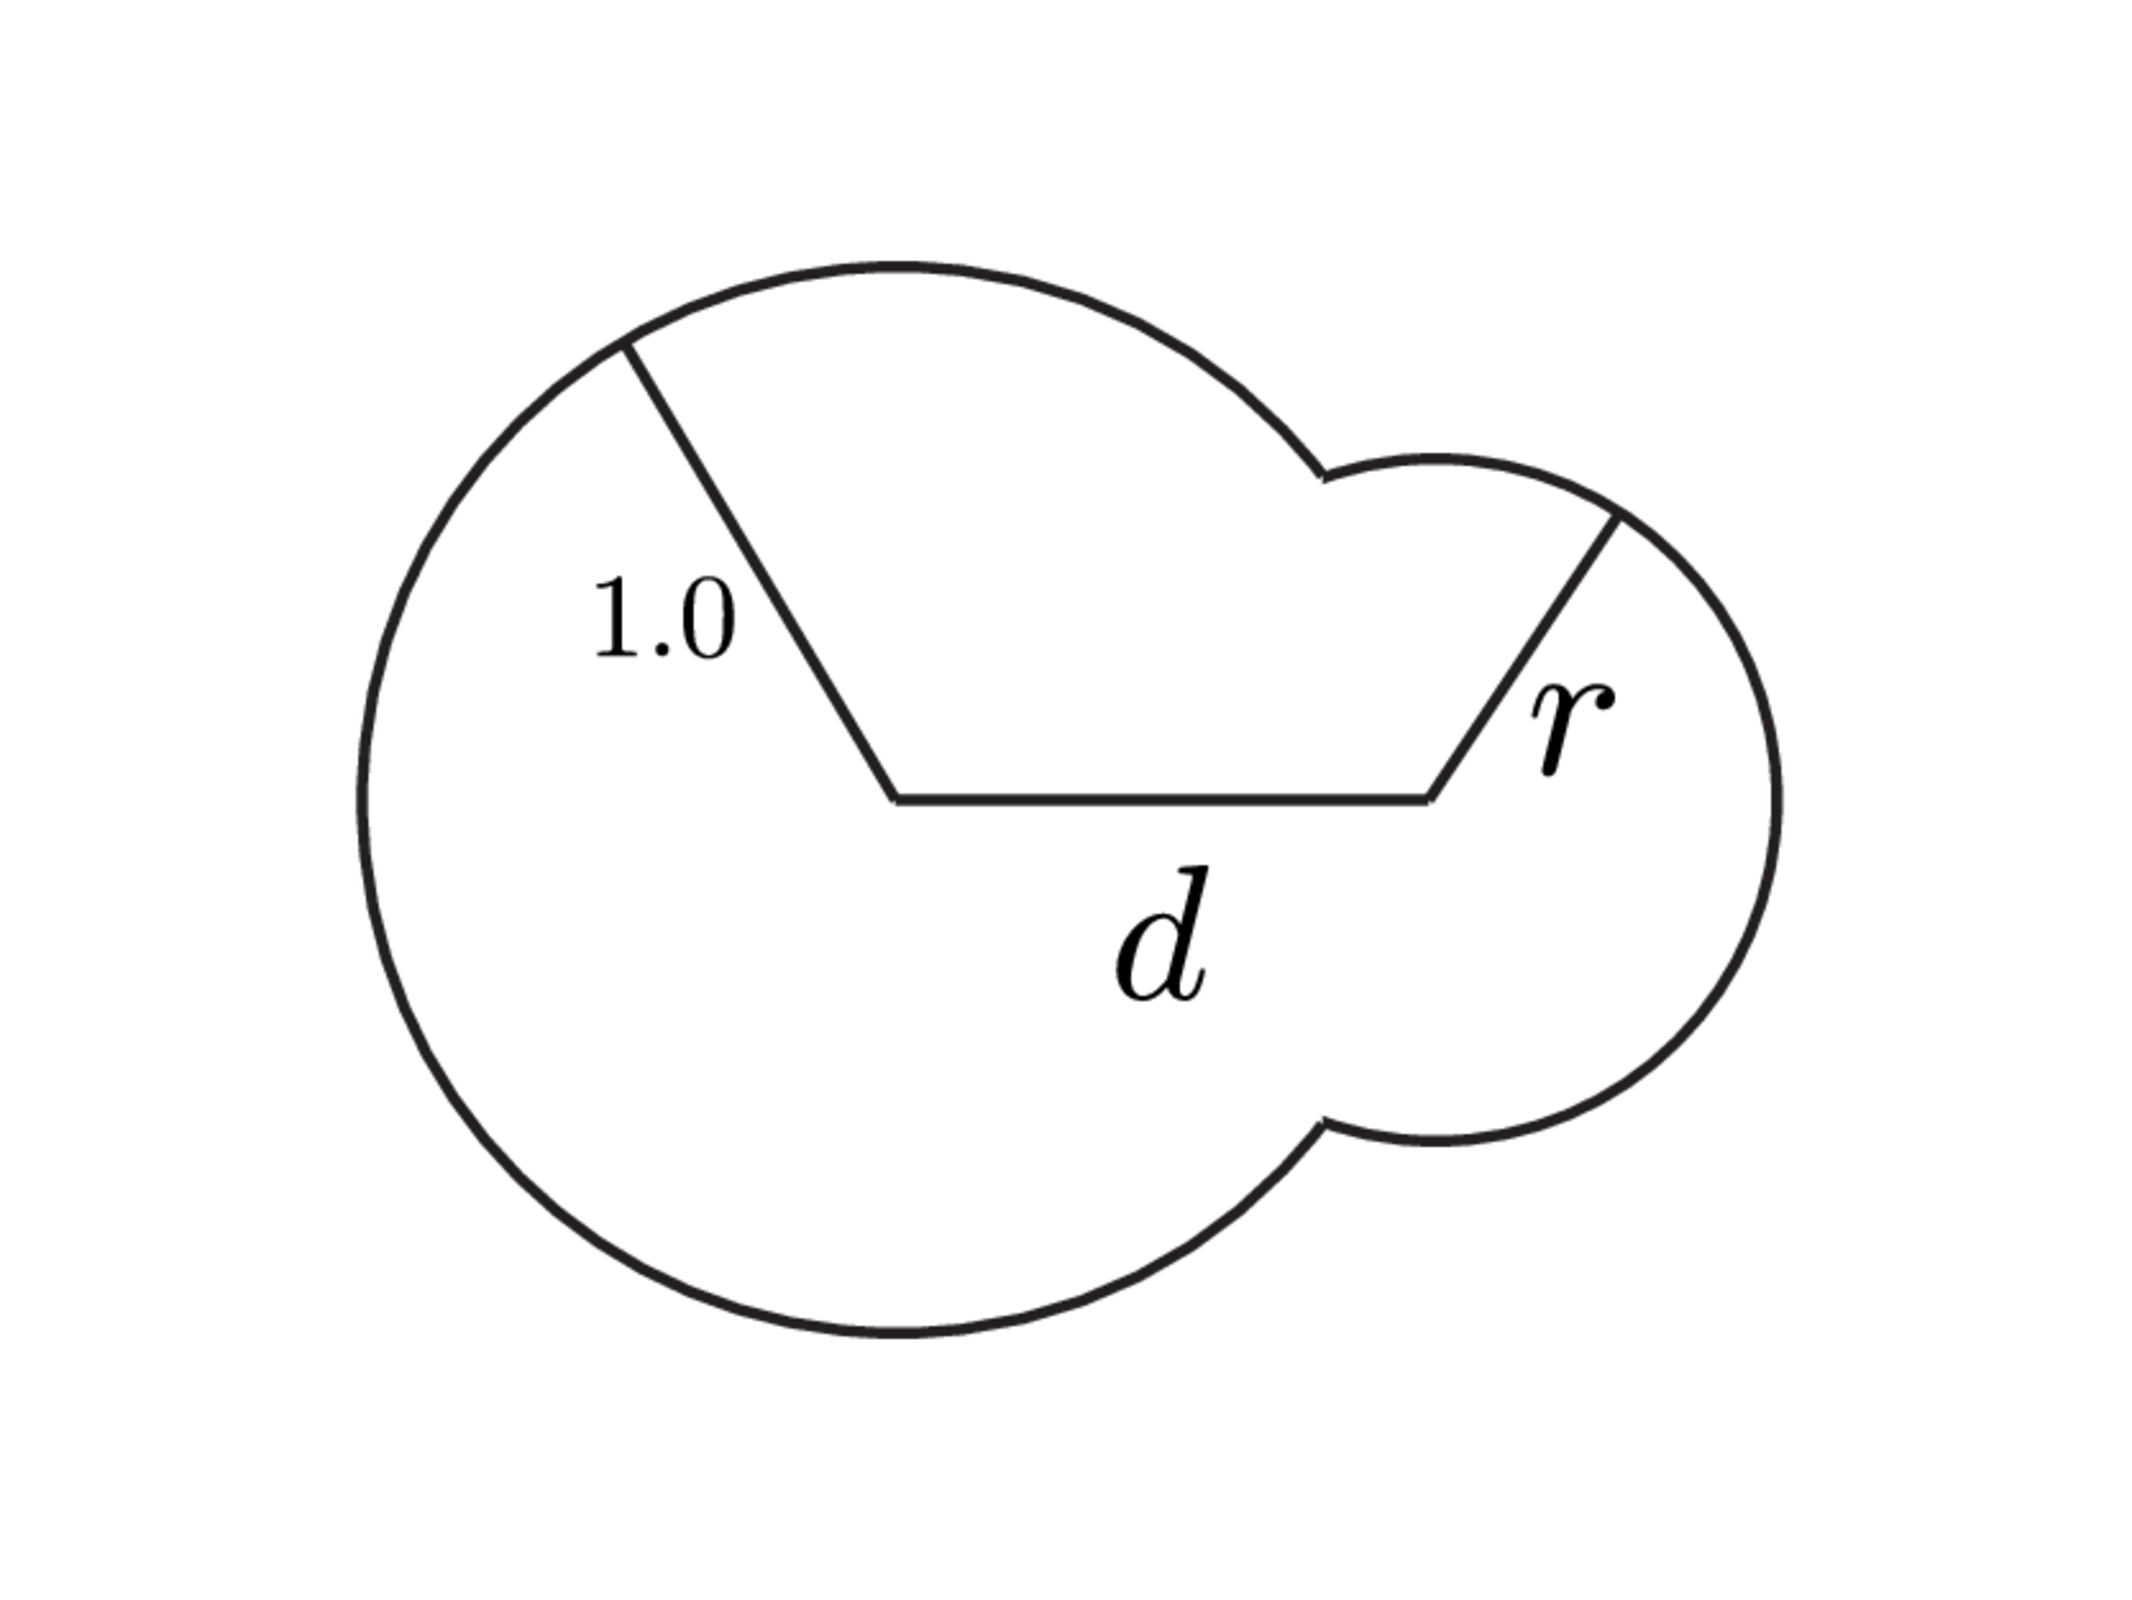
\includegraphics[width=\linewidth]{dimer}
        \caption{The Dimer molecule consists of a large particle of radius $1.0$, a small particle of radius $r$ separated by a distance $d$.}
        \label{fig:dimer}
    \end{subfigure}\hfill
    \begin{subfigure}[t]{0.48\textwidth}
        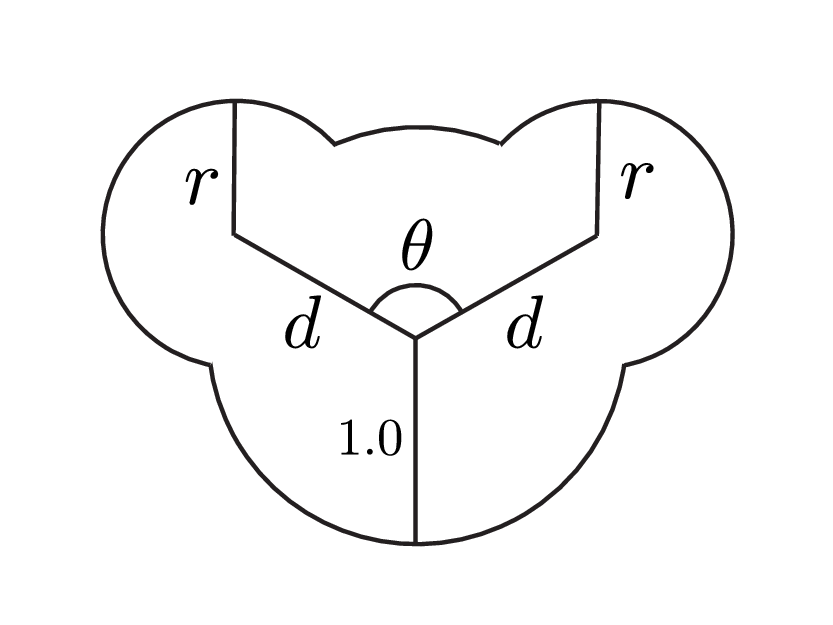
\includegraphics[width=\linewidth]{trimer}
        \caption{The Trimer molecule is comprised of a large particle of radius $1.0$ which subtends an angle $\theta$ between two small particles of radius $r$ at a distance $d$.}
        \label{fig:trimer}
    \end{subfigure}
    \caption{Construction of the molecules used in this thesis.}
    \label{fig:construction}
\end{figure}

The resulting collection of 50 molecules was cooled from a randomly generated high temperature state, resulting in a low temperature structure independent of the initial state. We assessed these low temperature structures for suitability on a number of criteria:
\begin{itemize}
    \item The molecules have to be resistant to crystallisation allowing long time dynamics to be characterised. There had to be no evidence of crystallisation in the low temperature structures.
    \item The molecules have to be radially definable allowing the use of the isopointal search algorithm developed by \textcite{hudson:10} to find the best packed structures as an approximation of the lowest energy structures.
    \item The concavity of the molecules should cover a wide range,
    \item The molecules have to be similar enough for direct comparison, and
    \item The molecules are representative of a wide range of molecular shapes.
\end{itemize}
The radius of 0.637556 is interesting as when combined with particles of radius $1.0$ it can form a compact packing~\appref{compact}. A dimer with a radius $r= 0.637556$ and a distance between the molecular centers $d= 1.637556$~\figref{dcon} hereafter denoted \dcon has a crystal structure that mirrors this compact packing. Despite \dcon having this well packed crystal structure, the low temperature state exhibited none of this crystal, indicating it is resilient to crystal formation. Retaining a radius of 0.637556 for the other molecules allows a more direct comparison, any differences are due to properties of the arrangement of particles, their shape, rather than the size ratios of the constituent particles. A distance $d= 1.0$ was chosen for another dimer~\figref{done} denoted \done and also for a trimer~\figref{tri} denoted \tri, for both consistency between the molecules and to allow all molecules to be described radially. An angle $\theta=120^\circ$ was chosen as this angle allows the maximum number of interparticle interactions for a trimer.

\begin{figure}
    \centering
    \captionsetup{justification=centering}
    \begin{subfigure}[t]{0.3\textwidth}
        \includegraphics[width=\linewidth]{{{Sone}}}
        \caption{$r=0.637556,$\\$d=1.0$ \\\done}
        \label{fig:done}
    \end{subfigure}\hfill
    \begin{subfigure}[t]{0.3\textwidth}
        \includegraphics[width=\linewidth]{{{Scon}}}
        \caption{$r=0.637556,$\\$d=1.637556$ \\\dcon}
        \label{fig:dcon}
    \end{subfigure}\hfill
    \begin{subfigure}[t]{0.3\textwidth}
        \includegraphics[width=\linewidth]{{{Tri}}}
        \caption{$r=0.637556,$\\$d=1.0, \theta=120 $\\\tri}
        \label{fig:tri}
    \end{subfigure}
    \caption[Molecules chosen for further study]{The molecules chosen for study in this thesis in order of the size of the concavity. The \done with the smallest concavity, \dcon with the smaller disc contacting the large disc and \tri which is a very similar to the \done molecule.}
    \label{fig:my mols}
\end{figure}

\section{Dynamics of \done}


With the main dynamical quantities of interest being the translation of the center of mass (COM) and the rotation. The measure of translational motion we are interested in is Mean Squared Displacement (MSD)~\figref{msd ex}. The MSD is given by
\begin{align}
    MSD(t) &= \langle \delta (t)^2 \rangle,\\
    \delta(t) &= \sqrt{(x(t) - x_0)^2 + (y(t) - y_0)^2}
    \label{eq:msd}
\end{align}
where $x(t)$ and $y(t)$ are the coordinates of the COM at time $t$, $x_0$ and $y_0$ are the initial coordinates of the molecule, and the angle brackets $\langle\,\rangle$ denote averaging over all molecules.

The MSD for \done over a range of temperatures is shown in \textfigref{snowman 0.637556 1.0 msd}. The initial region (\numrange{e-3}{e-1}) is the ballistic region where the particles are yet to collide with each other and are moving away from their initial position at constant velocity causing the MSD to increase as a $t^2$ power law. At high temperatures (\numrange{1.80}{3.50}) there is a direct transition from the ballistic to the diffusive regime, where the diffusive regime is defined by a MSD that increases as a linear function of $t$. In the diffusive regime the molecules are rearranging randomly. At lower temperatures (\num{0.90}) there is a distinct plateau between the ballistic and diffusive regimes. This plateau region is where there are only a small number of molecules that have escaped their local environment, most molecules still have the neighbours that they started with and are vibrating within the bounds of those neighbours.

\begin{figure}
    \centering
    \begin{subfigure}[t]{0.48\linewidth}
        \includegraphics[width=\textwidth]{{{msd}}}
        \caption{The mean squared displacement measures the distance the centers of mass ($\times$) move between the initial (grey) and final (black) positions.}
        \label{fig:msd ex}
    \end{subfigure}\hfill
    \begin{subfigure}[t]{0.48\linewidth}
        \includegraphics[width=\textwidth]{{{rot}}}
        \caption{The rotational relaxation measures how much molecules have rotated (black) from their initial position (grey) taking the dot product of the orientation vectors of each molecule.}
        \label{fig:rot ex}
    \end{subfigure}
    \begin{subfigure}{0.48\textwidth}
        \includegraphics[width=\textwidth]{{{struct}}}
        \caption{The structure function is a measure of how many particles have moved out of their initial positions (grey) with the threshold shown with a dotted green circle. Both rotational motion (depicted) and translational motion will result in particles moving out of this threshold region.}
        \label{fig:struct ex}
    \end{subfigure}
    \caption{A pictorial representation of the calculation of the mean squared displacement, rotational relaxation and structure function.}
    \label{fig:examples}
\end{figure} 

\begin{figure}
    \centering
    \begin{subfigure}[t]{0.48\linewidth}
        \includegraphics[width=\textwidth]{{{Snowman-0.637556-1.0-msd}}}
        \caption{Mean Squared Displacement, a measure of translational motion. The grey line indicates the $t^1$ power law defining the diffusive regime.}
        \label{fig:snowman 0.637556 1.0 msd}
    \end{subfigure}\hfill
    \begin{subfigure}[t]{0.48\linewidth}
        \includegraphics[width=\textwidth]{{{Snowman-0.637556-1.0-C_1}}}
        \caption{Rotational relaxation, a measure of rotational motion.}
        \label{fig:snowman 0.637556 1.0 r1}
    \end{subfigure}
    \begin{subfigure}{0.48\textwidth}
        \includegraphics[width=\textwidth]{{{Snowman-0.637556-1.0-F}}}
        \caption{Structure Function, a measure of structural relaxation.}
        \label{fig:snowman 0.637556 1.0 structure}
    \end{subfigure}
    \caption{The main dynamical features of the \done molecule over a range of temperatures, from a highly mobile liquid to a slow diffusive liquid.}
    \label{fig:snowman 0.637556 1.0}
\end{figure} 

The second dynamic quantity we are interested in is the rotational relaxation, a measure of the angular mobility of the molecule~\figref{rot ex}. The rotational relaxation $C_n(t)$ is given by
\begin{equation}
    C_n(t) = \langle P_n[\vect{\hat{e}}(0) \cdot \vect{\hat{e}}(t)] \rangle
    \label{eq:rot}
\end{equation}
where $P_n$ is the $n$\textsuperscript{th} order Legendre polynomial, $\vect{\hat{e}}(t)$ is the orientation vector at time $t$, and the angle brackets $\langle\,\rangle$ denote the averaging over all molecules. We are primarily interested in the first order rotational relaxation $C_1$ in which the Legendre polynomial takes the form
\begin{equation}
    P_1(x) = x
\end{equation}
however we do compare the first order function $C_1$ to the second order function $C_2$ later in this chapter to investigate the types of rotations that take place. The second order Legendre polynomial is given by
\begin{equation}
    P_2(x) = 2x^2 - 1
\end{equation}

The rotational relaxation for \done is given in \textfigref{snowman 0.637556 1.0 r1}. The rotational relaxation shows many features that are similar to the MSD, the initial period (\numrange{e-3}{e-1}) where the molecules have not had enough time to relax is constant at a value of \num{1}. Once past this initial region higher temperatures (\numrange{1.40}{3.50}) show a single exponential relaxation. At low temperatures (\numrange{0.9}{1.10}) there is a two step relaxation process, a small initial relaxation to a plateau region, followed by an exponential relaxation. This plateau region can be explained in the same way as the plateau in the MSD, the molecules are vibrating within local structures.

The third dynamical quantity that we were interested in is the Structure Function $F(t)$~\figref{struct ex}. The Structure function is different from the MSD and Rotational relaxations in that instead of calculating quantities for each molecule and averaging over all molecules, the values are calculated for each particle of each molecule and averaged over all the particles. The Structure function is given by
\begin{align}
    F(t) = \left \langle \begin{cases}
        \quad0 &\text{if}\quad \delta > 0.3 \\
        \quad1 &\text{if}\quad \delta \leq 0.3
    \end{cases} \quad \right \rangle
    \label{eq:struct}
\end{align}
where $\delta$ is the distance of each particle from its initial position~\eqref{msd} and the angle brackets $\langle\,\rangle$ denote averaging over all particles. The value of \num{0.3} was chosen to be small enough to be able to observe the combination of translational and rotational motion of a molecule.

The Structure function for \done is shown in \textfigref{snowman 0.637556 1.0 structure} and shows some interesting characteristics. The initial region (\numrange{e-3}{e-1}) is flat where the particles have not had enough time to move a distance of \num{0.3} units. The sharp dropoff (\numrange{e-1}{1e0}), characteristic of the binary function, occurs at the same time the MSD transitions from the ballistic regime showing the molecules escaping their local environment.

\section{Dynamics of \dcon and \tri}

The dynamics of the \dcon \figref{dcon dynamics} and \tri~\figref{tri dynamics} molecules show similar behaviour to the \done molecule. The most noticeable difference is the temperature at which the dynamics slow down, in the \done molecule we collect dynamic quantities down to a temperature of \num{0.90}, for the \dcon molecule we are only able to get results down to \num{1.75} and the \tri molecule down to \num{1.15}. We are unable to characterise the dynamics below these temperature as the dynamical quantities become too slow to characterise. The dramatic change in low temperature behaviour for relatively small changes in molecular shape is a result that we investigate further throughout the rest of this thesis.

Apart from the dramatic differences in temperature the dynamics exhibits similar behaviour. The MSD of both \dcon \figref{snowman 0.637556 1.637556 msd} and \tri \figref{trimer 0.637556 1.0 120 msd} show the same levelling out at low temperature in the region between the short time ballistic regime (\numrange{e-3}{e-1}) and the long time diffusive regime (\numrange{e3}{e6}). The rotational relaxations and structure functions also show the same two step relaxations as the \done molecule, however the initial relaxation is a much smaller relaxation. One of the differences in behaviour is in the structure function of \tri~\figref{trimer 0.637556 1.0 120 structure}, where there is a more obvious plateau containing oscillations. These oscillations are the result of small correlated motions of particles such that they oscillate in and out of the cutoff distance.

\begin{figure}
    \centering
    \begin{subfigure}[t]{0.45\linewidth}
        \includegraphics[width=\textwidth]{{{Snowman-0.637556-1.637556-msd}}}
        \caption{Mean Squared Displacement, a measure of translational motion. The grey line indicates the $t^1$ power law defining the diffusive regime.}
        \label{fig:snowman 0.637556 1.637556 msd}
    \end{subfigure}
    \begin{subfigure}[t]{0.45\linewidth}
        \includegraphics[width=\textwidth]{{{Snowman-0.637556-1.637556-C_1}}}
        \caption{Rotational relaxation, a measure of rotational motion.}
        \label{fig:snowman 0.637556 1.637556 r1}
    \end{subfigure}
    \begin{subfigure}{0.45\textwidth}
        \includegraphics[width=\textwidth]{{{Snowman-0.637556-1.637556-F}}}
        \caption{Structure function, a measure of structural relaxation.}
        \label{fig:snowman 0.637556 1.637556 structure}
    \end{subfigure}
    \caption{The dynamics of the \dcon molecule over a range of temperatures. The range of temperatures is smaller than that of the \done molecule due to the slower dynamics of the \dcon molecule at low temperatures.}
    \label{fig:dcon dynamics}
\end{figure}

\begin{figure}
    \centering
    \begin{subfigure}[t]{0.45\linewidth}
        \includegraphics[width=\textwidth]{{{Trimer-0.637556-1.00-120-msd}}}
        \caption{Mean Squared Displacement, a measure a translational motion. The grey line indicates the $t^1$ power law defining the diffusive regime.}
        \label{fig:trimer 0.637556 1.0 120 msd}
    \end{subfigure}\hfill
    \begin{subfigure}[t]{0.45\linewidth}
        \includegraphics[width=\textwidth]{{{Trimer-0.637556-1.00-120-C_1}}}
        \caption{Rotational relaxation, a measure of rotational motion.}
        \label{fig:trimer 0.637556 1.0 120 r1}
    \end{subfigure}
    \begin{subfigure}{0.45\textwidth}
        \includegraphics[width=\textwidth]{{{Trimer-0.637556-1.00-120-F}}}
        \caption{Structure function, a measure of structural relaxation.}
        \label{fig:trimer 0.637556 1.0 120 structure}
    \end{subfigure}
    \caption{Dynamics of the \tri molecule across a range of temperatures.}
    \label{fig:tri dynamics}
\end{figure}

\section{Comparison of Dynamic Quantities}

The functions that we have dealt with so far allow a comparison of the behaviour of a molecule over a range of temperatures, what we are unable to do is easily compare molecules and be able to interpret all the data on a single plot. To make comparisons we want to represent each function as a single value. For the MSD we can use the diffusion constant, found as,
\begin{equation}
    D = \frac{1}{4}\ddiff{\,MSD(t)}{t}
\end{equation} 
a multiple of the gradient. The gradient of the MSD from which the diffusion constant is defined is in the diffusive region. To get an accurate value of the diffusion constant the average value of the gradient was calculated for this region. The rotational relaxation and the structure function are functions with similar characteristics and can be treated in the same way. We can define relaxation times $\tau_1,\tau_2,\text{and},\tau_s$ as the time for these functions to reach a specific value. The exponentially decaying nature of the rotational relaxation and structure functions makes the value of $1/\e$ relevant since the time $t$ is related to the exponential factor $k$ by the relation $k=1/t$.

Comparing the dynamic quantities of the three molecules~\figref{dynamic comparison} there are large differences between the molecules. Looking at the diffusion constant~\figref{D}, \done shows a linear decrease in the diffusion constant as the temperature decreases. This linear behaviour is consistent with the Arrhenius relation and indicates that the molecular rearrangements that take place have a constant activation energy. The \dcon molecule shows definite non Arrhenius behaviour, with the diffusion constant diverging from that of \done by more than two orders of magnitude, while the \tri molecule tracks between the \done and \dcon molecules. Both the rotational relaxation~\figref{t1} and structural relaxation~\figref{ts} show similar behaviour to the diffusion constant, \done shows linear temperature dependence, the behaviour of a strong glass forming liquid. The \dcon molecule exhibits a significant increase as the temperature decreases, the behaviour of a fragile liquid. The final molecule, \tri sits between the \done and the \dcon molecules covering the range of dynamic behaviour of liquids.

The structural relaxation~\figref{ts} displays two gradients for each of the molecules, indicative of two separate relaxation processes with different activation energies. At high temperatures there is a process with a low activation energy which suddenly transitions at low temperatures to a process with a high activation energy. Neither the diffusion constant or the rotational relaxation show this sudden transition between two processes. By multiplying the diffusion constant~$D$ by the structural relaxation time~$\tau_s$ \figref{D.ts} the change in relaxation process is clearly seen as the inflection point. Initially the structural relaxation is dominated by translational motion, a process with a low activation energy. However at the inflection point the process changes to one dominated by rotational motion with at higher activation energy. Further evidence of this transition is comparing the activation energies of the rotational~\figref{t1} and structural~\figref{ts} relaxations, after the transition of the structural relaxation to a rotationally dominated process the activation energies show strong correlations. Despite the sudden change in the structural relaxation time, there is no corresponding discontinuity in the diffusion constant~\figref{D}. In defining the diffusion constant we are only interested in the gradient of the MSD in the diffusive regime, ignoring the time to reach the diffusive regime. At low temperatures the plateau region of the MSD is sits below the 0.09 cutoff of the structure function, during which rotations are the primary contributor to the structural relaxation. 

\begin{figure}
    \centering
    \begin{subfigure}{\linewidth}
        \centering
        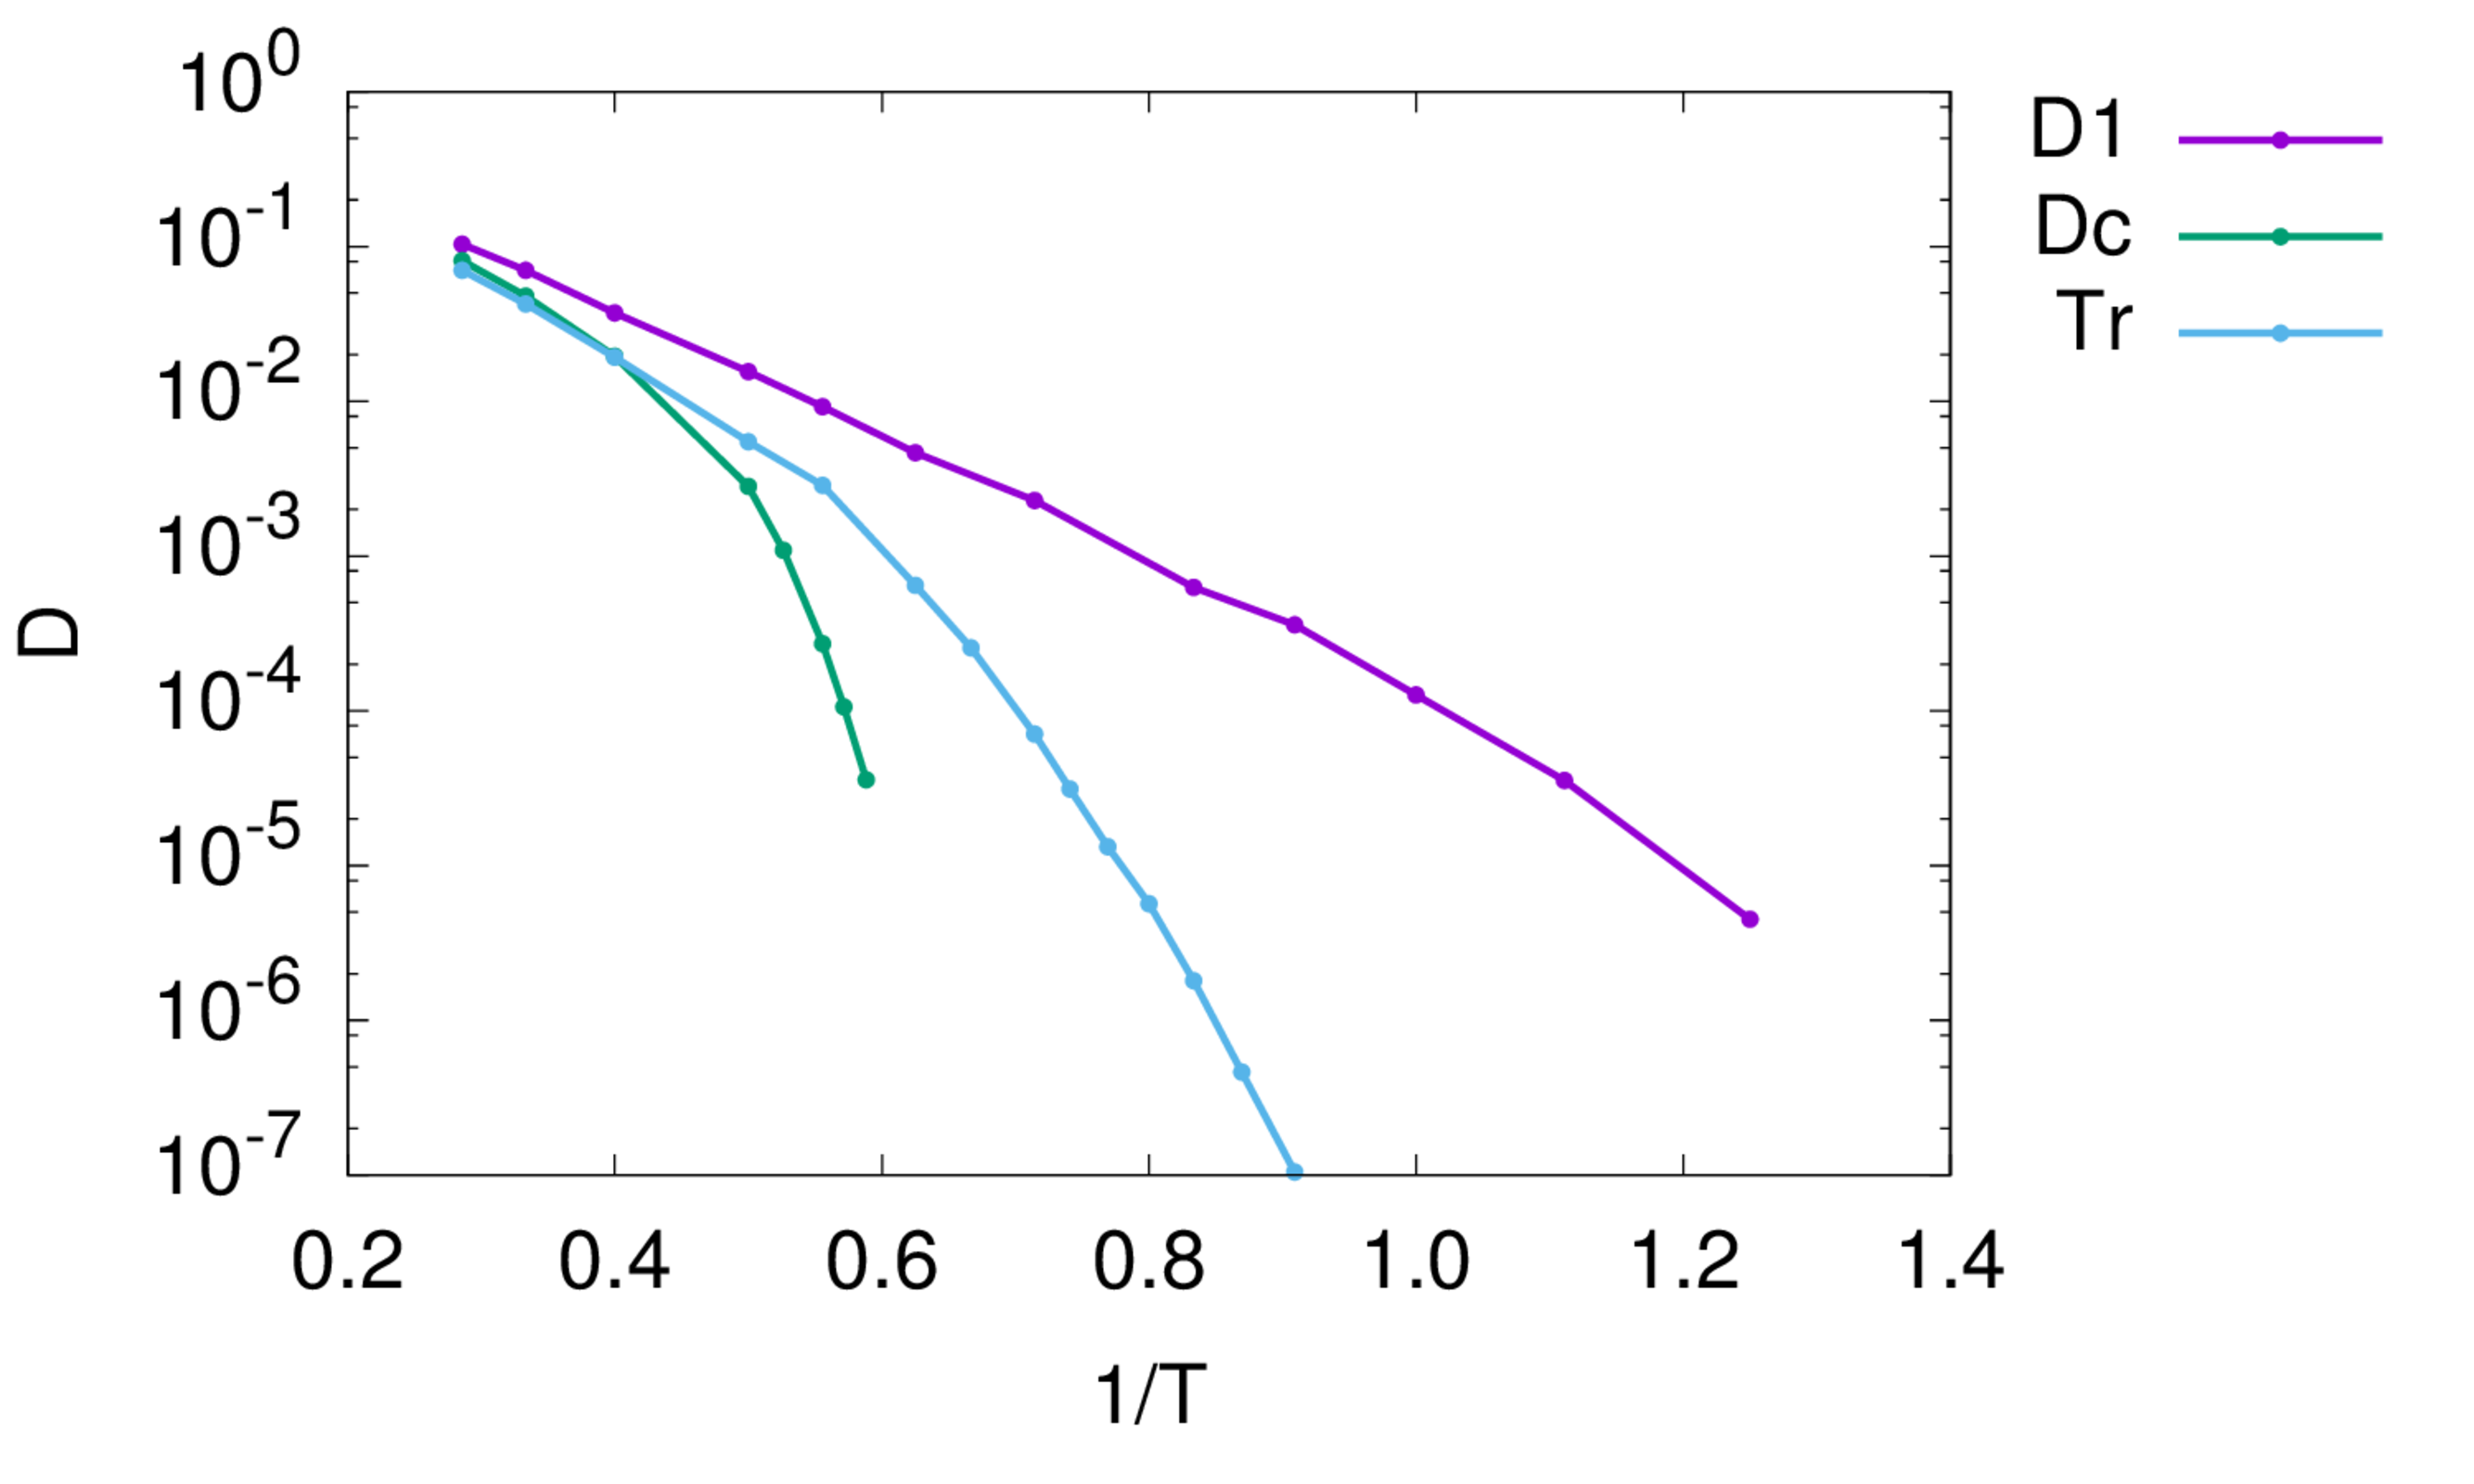
\includegraphics[width=0.6\textwidth]{D}
        \caption{Comparison of the diffusion constant of the three molecules over a range of temperatures. The \done molecule has a diffusion constant that is linear, while the \tri and \dcon exhibit increasingly fragile behaviour.}
        \label{fig:D}
    \end{subfigure}
    \begin{subfigure}{\linewidth}
        \centering
        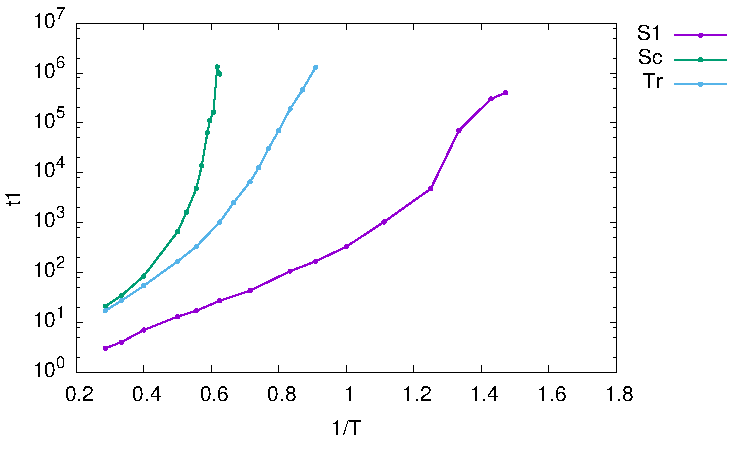
\includegraphics[width=0.6\textwidth]{t1}
        \caption{Comparison of rotational relaxation times of the three molecules over a range of temperatures. The activation energies of the processes at low temperatures are shown by fitting an exponential to these regions.}
        \label{fig:t1}
    \end{subfigure}
    \begin{subfigure}{\textwidth}
        \centering
        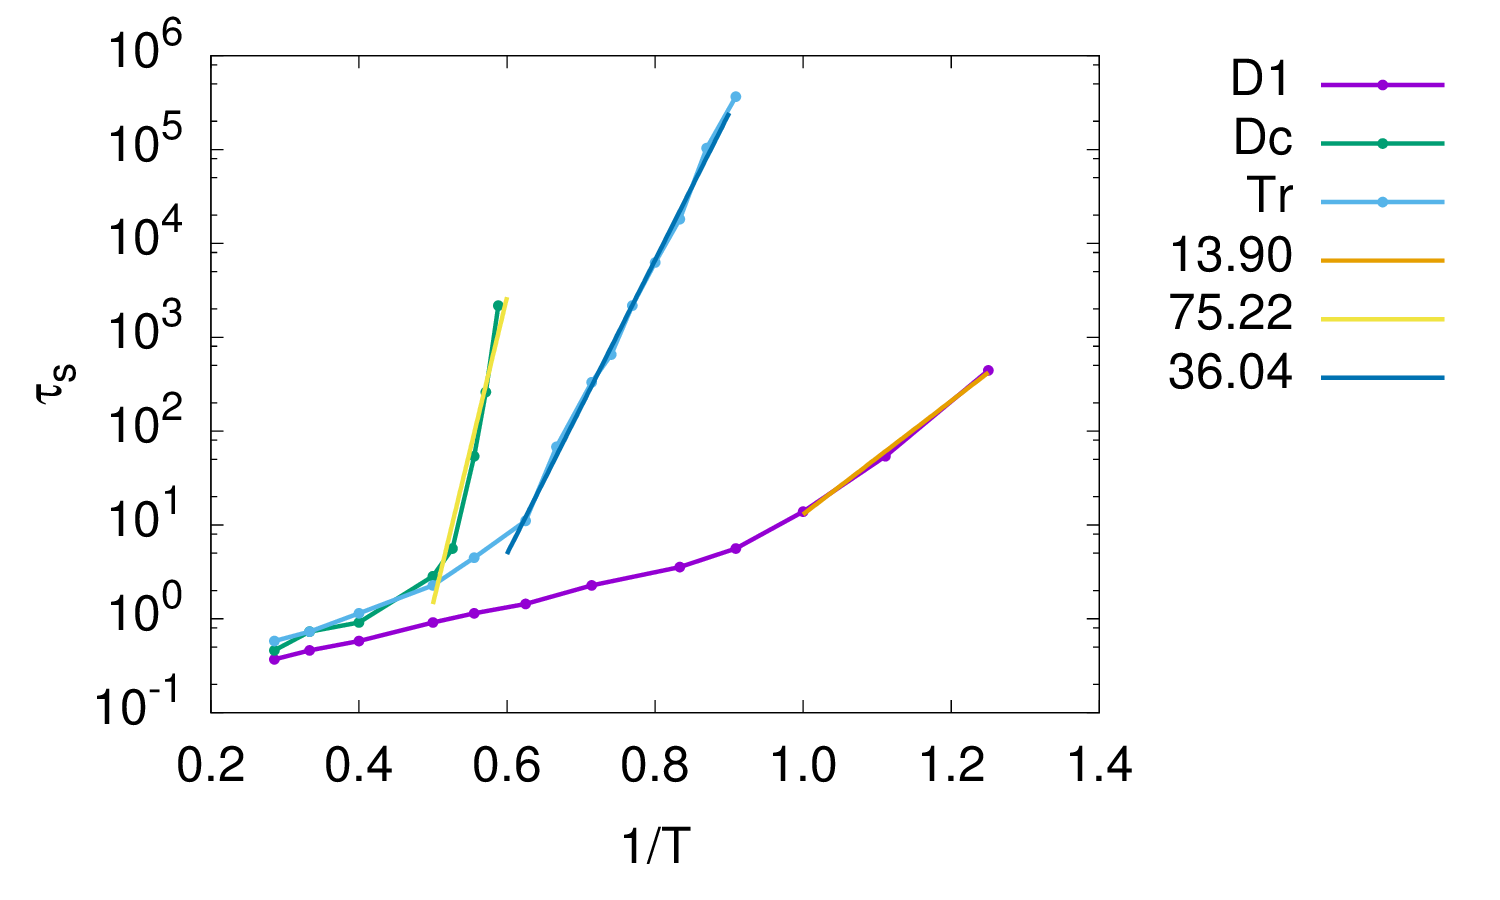
\includegraphics[width=0.6\textwidth]{ts}
        \caption{Comparison of the structural relaxation time for the three molecules over a range of temperatures. There is a sharp transition in these functions giving a high and low temperature regions. The activation energies of the low temperature regions are shown by fitting exponentials to these regions.}
        \label{fig:ts}
    \end{subfigure}
    \caption{Comparison of the diffusion constant, rotational relaxation time $\tau_1$ and structural relaxation time $\tau_s$ for the three molecules that we are studying. Small changes to shape result in changes of many orders of magnitude to dynamic quantities.}
    \label{fig:dynamic comparison}
\end{figure}

\begin{figure}
    \centering
    \includegraphics[width=0.6\textwidth]{{{D.ts}}}
    \caption{Relative contribution of diffusion to structural relaxation over a number of temperatures. The discontinuity shows the point at which the structural relaxation moves from being dominated by translational motion to being dominated by rotational motion.}
    \label{fig:D.ts}
\end{figure}

The increased contribution of the rotations to the overall dynamics is an interesting result, previous studies both experimental~\cite{stillinger:94,cicerone:95,debenedetti:01,swallen:03} and simulated~\cite{kammerer:97} have found that translations, rather than rotations dominate at low temperatures contrary to our observations of structural relaxations. Further support for the dominance of rotations in our systems is seen by taking the product of the diffusion constant and the rotational relaxation~\figref{D.t1}, the diffusion constant is getting smaller much faster than the increase in the rotational relaxation time. One possible explanation for the dominance of rotations over translations at low temperature is that when molecules interlock via a concavity the concavity inhibits the translational motion, molecules have to unlock from the concavity to move past one another. Rotations however, are possible while still retaining the interaction at the concavity.

\begin{figure}
    \centering
    \includegraphics[width=0.6\textwidth]{{{D.t1}}}
    \caption{Relative contributions of the diffusion constant and rotational relaxation to the overall dynamics. The decrease as the temperature decreased indicates the translational diffusion is getting slower faster than the rotational diffusion.}
    \label{fig:D.t1}
\end{figure}

Studying the rotations of our molecules further, results found in simulations of similar molecules~\cite{kammerer:97,michele:01} found that at low temperatures molecules underwent rotational relaxation by flips of \ang{180}. To investigate the contribution of \ang{180} jumps in our molecules we can compare the first and second order rotational relaxation times since flips of \ang{180} do not contribute to the second order relaxation. Taking the ratio of the first and second relaxation times $\tau_1/\tau_2$ we can determine whether these \ang{180} are present in our simulations~\figref{t1/t2}. We see a decrease in this ratio for all molecules, $\tau_2$ is larger than $\tau_1$ at low temperature meaning there is little contribution to the relaxation be \ang{180} flips in orientation.

\begin{figure}
    \centering
    \includegraphics[width=0.6\textwidth]{{{t1.t2}}}
    \caption{The ratio of the first and second order rotational relaxation times as a function of temperature. As the temperature decreases the decrease in this ratio shows that molecules undergo small angle changes rather than \ang{180} flips.}
    \label{fig:t1/t2}
\end{figure}

In describing the differences between the dynamic properties of the molecules the Aperiodic Crystal Structure model provides a relationship between the rotational relaxation and the diffusion constant and the local structural rigidity in the Hall-Wolynes equation~\cite{hall:87,dyre:96}
\begin{equation}
    \tau_1, D \propto \e^{a^2/2\langle u^2\rangle}
\end{equation}
where $a$ is the displacement to overcome the local energy barrier and $\langle u^2 \rangle$ is the Debye-Waller factor, a measure of the local rigidity of the structure. The Debye-Waller factor is found as the MSD at the time where 
\begin{equation}
    \ddiff{\log{(\text{MSD})}}{\log{(t)}}
\end{equation}
is a minimised~\cite{larini:08}, the value where the slope is lowest in \textfigref{snowman 0.637556 1.0 msd}.

Plotting the diffusion constant~\figref{DW.D} and the rotational relaxation time~\figref{DW.t1} against $1/\langle u^2 \rangle$ we see that instead of the molecules diverging there is a much better correlation between them. The Debye-Waller factor normalises the dynamics based on the local structural rigidity explaining a significant portion of the difference in the dynamics of the molecules. In changing the shape of molecules we change the local stiffness of the liquid phase resulting in order of magnitude changes of the dynamics. The cause of the temperature dependence of the local stiffness is likely a key contributor to the fragility of a liquid.

\begin{figure}
    \begin{subfigure}{\textwidth}
        \centering
        \includegraphics[width=0.6\textwidth]{{{DW.D}}}
        \caption{At high temperatures the Debye-Waller factor $\langle u^2 \rangle$ is a fairly constant large value (left of figure). As the temperature decreases all molecules show diffusion constants over an order of magnitude range at any value of $\langle u^2 \rangle$, much smaller than the four orders of magnitude when plotting against temperature.}
        \label{fig:DW.D}
    \end{subfigure}
    \begin{subfigure}{\textwidth}
        \centering
        \includegraphics[width=0.6\textwidth]{{{DW.t1}}}
        \caption{At high temperatures the Debye-Waller factor $\langle u^2 \rangle$ is a fairly constant large value (left of figure). As the temperature decreases both \done and \tri show similar rotational relaxation times. The \dcon molecule shows a steeper slope indicating the presence of more complicated process.}
        \label{fig:DW.t1}
    \end{subfigure}
    \caption{By normalising the diffusion constant and rotational relaxation by the Debye-Waller factor we are able to account for a significant portion of large differences in the dynamic quantities.}
\end{figure}
